\tikzset{every picture/.style={line width=0.75pt}} %set default line width to 0.75pt        
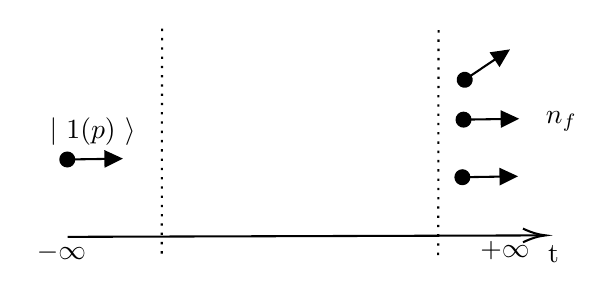
\begin{tikzpicture}[x=0.75pt,y=0.75pt,yscale=-1,xscale=1]
%uncomment if require: \path (0,194); %set diagram left start at 0, and has height of 194

%Straight Lines [id:da28910037002363764] 
\draw    (205.27,107.68) -- (433.59,106.98) ;
\draw [shift={(435.59,106.97)}, rotate = 539.8199999999999] [color={rgb, 255:red, 0; green, 0; blue, 0 }  ][line width=0.75]    (10.93,-3.29) .. controls (6.95,-1.4) and (3.31,-0.3) .. (0,0) .. controls (3.31,0.3) and (6.95,1.4) .. (10.93,3.29)   ;
%Straight Lines [id:da7985070919800723] 
\draw  [dash pattern={on 0.84pt off 2.51pt}]  (250.78,7.4) -- (250.61,116.64) ;
%Straight Lines [id:da47959589803581304] 
\draw  [dash pattern={on 0.84pt off 2.51pt}]  (383.98,8.11) -- (383.81,117.35) ;
%Straight Lines [id:da17940445023321017] 
\draw    (205.1,70.41) -- (228.91,70.04) ;
\draw [shift={(231.91,69.99)}, rotate = 539.0899999999999] [fill={rgb, 255:red, 0; green, 0; blue, 0 }  ][line width=0.08]  [draw opacity=0] (8.93,-4.29) -- (0,0) -- (8.93,4.29) -- cycle    ;
\draw [shift={(205.1,70.41)}, rotate = 359.09] [color={rgb, 255:red, 0; green, 0; blue, 0 }  ][fill={rgb, 255:red, 0; green, 0; blue, 0 }  ][line width=0.75]      (0, 0) circle [x radius= 3.35, y radius= 3.35]   ;
%Straight Lines [id:da9397044962896224] 
\draw    (396.57,32.01) -- (415.9,19.03) ;
\draw [shift={(418.39,17.36)}, rotate = 506.11] [fill={rgb, 255:red, 0; green, 0; blue, 0 }  ][line width=0.08]  [draw opacity=0] (8.93,-4.29) -- (0,0) -- (8.93,4.29) -- cycle    ;
\draw [shift={(396.57,32.01)}, rotate = 326.11] [color={rgb, 255:red, 0; green, 0; blue, 0 }  ][fill={rgb, 255:red, 0; green, 0; blue, 0 }  ][line width=0.75]      (0, 0) circle [x radius= 3.35, y radius= 3.35]   ;
%Straight Lines [id:da4306245684857515] 
\draw    (395.46,78.95) -- (419.27,78.57) ;
\draw [shift={(422.27,78.52)}, rotate = 539.0899999999999] [fill={rgb, 255:red, 0; green, 0; blue, 0 }  ][line width=0.08]  [draw opacity=0] (8.93,-4.29) -- (0,0) -- (8.93,4.29) -- cycle    ;
\draw [shift={(395.46,78.95)}, rotate = 359.09] [color={rgb, 255:red, 0; green, 0; blue, 0 }  ][fill={rgb, 255:red, 0; green, 0; blue, 0 }  ][line width=0.75]      (0, 0) circle [x radius= 3.35, y radius= 3.35]   ;
%Straight Lines [id:da8816879387506134] 
\draw    (396.02,51.21) -- (419.83,50.83) ;
\draw [shift={(422.83,50.78)}, rotate = 539.0899999999999] [fill={rgb, 255:red, 0; green, 0; blue, 0 }  ][line width=0.08]  [draw opacity=0] (8.93,-4.29) -- (0,0) -- (8.93,4.29) -- cycle    ;
\draw [shift={(396.02,51.21)}, rotate = 359.09] [color={rgb, 255:red, 0; green, 0; blue, 0 }  ][fill={rgb, 255:red, 0; green, 0; blue, 0 }  ][line width=0.75]      (0, 0) circle [x radius= 3.35, y radius= 3.35]   ;


% Text Node
\draw (443.19,51.92) node    {$n_{f}$};
% Text Node
\draw (217.31,56.9) node    {$|\ 1( p) \ \rangle $};
% Text Node
\draw (439.31,115.93) node   [align=left] {t};
% Text Node
\draw (202.32,115.22) node    {$-\infty $};
% Text Node
\draw (416,114.51) node    {$+\infty $};

\end{tikzpicture}